\documentclass[12pt]{article}
\usepackage{geometry}                % See geometry.pdf to learn the layout options. There are lots.
\geometry{letterpaper}                   % ... or a4paper or a5paper or ... 
%\geometry{landscape}                % Activate for for rotated page geometry
\usepackage[parfill]{parskip}    % Activate to begin paragraphs with an empty line rather than an indent
\usepackage{daves,fancyhdr,natbib,graphicx,dcolumn,amsmath,lastpage,url}
\usepackage{amsmath,amssymb,epstopdf,longtable}
\usepackage{paralist} 
\DeclareGraphicsRule{.tif}{png}{.png}{`convert #1 `dirname #1`/`basename #1 .tif`.png}
\pagestyle{fancy}
\lhead{CE 3372 -- Water Systems Design}
\rhead{SPRING 2025}
\lfoot{EXERCISE 5}
\cfoot{}
\rfoot{Page \thepage\ of \pageref{LastPage}}
\renewcommand\headrulewidth{0pt}
\newcommand\tab[1][1cm]{\hspace*{#1}}


\begin{document}
\begin{center}
{\textbf{{ CE 3372 -- Water Systems Design} \\ {Exercise Set 6}}}
\end{center}
\begingroup
\begin{tabular}{p{1in} p{5in}}
Purpose: & Demonstrate flow-equalization volume required for a storage tank to leverage some constant flow rate.\\
Task(s): & Analyze daily water cumulative demand (from time varying outflows) \\
~ & Find equivalent constant draw rate \\
~ &  Use double mass curve concept to find maximum deviations to size an equalization tank.\\
\end{tabular}
\endgroup
\section*{\small{Exercise}}
\begin{enumerate}
%%%%%%%%%%%%%%%%%%%%%%%%%%%%%%%%%%%%%%%%%%%%%%%%%%%%%%%
%%%%%%%%%%%%%%% PROBLEM 1 %%%%%%%%%%%%%%%%%%%%%%%%%%%%

\item Figure \ref{fig:DraftCurve} is a plot of variable cumulative inflow volume versus time for a proposed flow-equalization tank location and the equivalent constant rate inflow for the same location. 

\begin{figure}[h!] %  figure placement: here, top, bottom, or page
\centering
   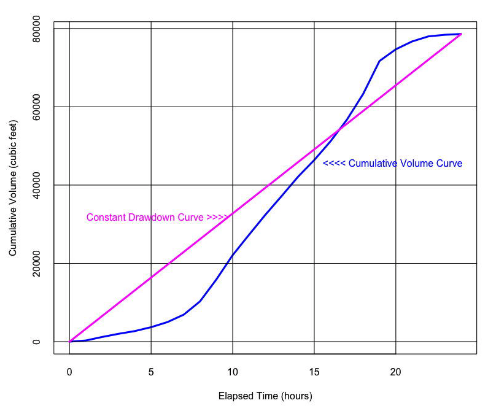
\includegraphics[width=5in]{DraftCurve.png}
   \caption{Time-varying water demand (cumulative) and constant-rate equivalent demand }
   \label{fig:DraftCurve} 
\end{figure}

\clearpage

Figure \ref{fig:DraftTable} is a list of time and cumulative volume inflow (same as the graph). A flow-equalization storage tank volume is to be determined.

\begin{figure}[h!] %  figure placement: here, top, bottom, or page
\centering
   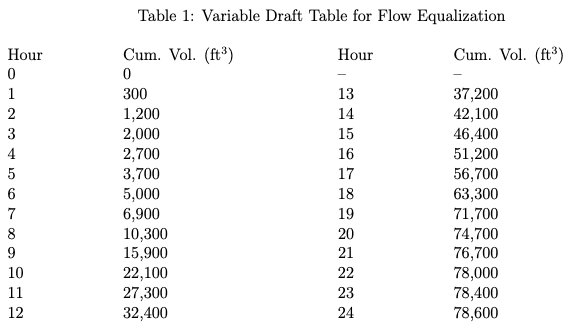
\includegraphics[width=5in]{DraftTable.png}
   \caption{Variable Draft Table for Flow Equalization }
   \label{fig:DraftTable} 
\end{figure}

Determine:
\begin{enumerate}
\item The cumulative volume of inflow (or draft) every 24 hours plotted on Figure \ref{fig:DraftCurve} and tabulated in Figure \ref{fig:DraftTable}.
\item The constant flow rate (cubic feet per hour) from the constant drawdown curve plotted on Figure \ref{fig:DraftCurve} and tabulated in Figure \ref{fig:DraftTable}.
\item The largest maximum absolute deviation between the constant drawdown line and the variable inflow curve indicated by Figure \ref{fig:DraftCurve} and/or tabulated in Figure \ref{fig:DraftTable}.
\item The second largest maximum absolute deviation between the constant drawdown line and the variable inflow curve indicated by Figure \ref{fig:DraftCurve} and/or tabulated in Figure \ref{fig:DraftTable}.
\item A recommended flow equalization storage volume indicated by Figure \ref{fig:DraftCurve} and/or tabulated in Figure \ref{fig:DraftTable}.
\end{enumerate}
\end{enumerate}
\begin{thebibliography}{}
%
\bibitem[\protect\citeauthoryear{Gupta2017}{Gupta}{2017}]{Gupta2017}
Gupta, R. S. 2017. Hydrology and Hydraulic Systems. Waveland Press, Inc. pp. 548-552
%
%
\end{thebibliography}
\end{document}  